\documentclass[11pt,a4paper,]{article}
\usepackage{lmodern}

\usepackage{amssymb,amsmath}
\usepackage{ifxetex,ifluatex}
\usepackage{fixltx2e} % provides \textsubscript
\ifnum 0\ifxetex 1\fi\ifluatex 1\fi=0 % if pdftex
  \usepackage[T1]{fontenc}
  \usepackage[utf8]{inputenc}
\else % if luatex or xelatex
  \usepackage{unicode-math}
  \defaultfontfeatures{Ligatures=TeX,Scale=MatchLowercase}
\fi
% use upquote if available, for straight quotes in verbatim environments
\IfFileExists{upquote.sty}{\usepackage{upquote}}{}
% use microtype if available
\IfFileExists{microtype.sty}{%
\usepackage[]{microtype}
\UseMicrotypeSet[protrusion]{basicmath} % disable protrusion for tt fonts
}{}
\PassOptionsToPackage{hyphens}{url} % url is loaded by hyperref
\usepackage[unicode=true]{hyperref}
\hypersetup{
            pdftitle={ETC513 Assignment 3: Comparison of Energy and Pollution by Country},
            pdfborder={0 0 0},
            breaklinks=true}
\urlstyle{same}  % don't use monospace font for urls
\usepackage{geometry}
\geometry{a4paper, centering, text={16cm,24cm}}
\usepackage[style=authoryear-comp,]{biblatex}
\addbibresource{references.bib}
\usepackage{color}
\usepackage{fancyvrb}
\newcommand{\VerbBar}{|}
\newcommand{\VERB}{\Verb[commandchars=\\\{\}]}
\DefineVerbatimEnvironment{Highlighting}{Verbatim}{commandchars=\\\{\}}
% Add ',fontsize=\small' for more characters per line
\usepackage{framed}
\definecolor{shadecolor}{RGB}{248,248,248}
\newenvironment{Shaded}{\begin{snugshade}}{\end{snugshade}}
\newcommand{\AlertTok}[1]{\textcolor[rgb]{0.94,0.16,0.16}{#1}}
\newcommand{\AnnotationTok}[1]{\textcolor[rgb]{0.56,0.35,0.01}{\textbf{\textit{#1}}}}
\newcommand{\AttributeTok}[1]{\textcolor[rgb]{0.77,0.63,0.00}{#1}}
\newcommand{\BaseNTok}[1]{\textcolor[rgb]{0.00,0.00,0.81}{#1}}
\newcommand{\BuiltInTok}[1]{#1}
\newcommand{\CharTok}[1]{\textcolor[rgb]{0.31,0.60,0.02}{#1}}
\newcommand{\CommentTok}[1]{\textcolor[rgb]{0.56,0.35,0.01}{\textit{#1}}}
\newcommand{\CommentVarTok}[1]{\textcolor[rgb]{0.56,0.35,0.01}{\textbf{\textit{#1}}}}
\newcommand{\ConstantTok}[1]{\textcolor[rgb]{0.00,0.00,0.00}{#1}}
\newcommand{\ControlFlowTok}[1]{\textcolor[rgb]{0.13,0.29,0.53}{\textbf{#1}}}
\newcommand{\DataTypeTok}[1]{\textcolor[rgb]{0.13,0.29,0.53}{#1}}
\newcommand{\DecValTok}[1]{\textcolor[rgb]{0.00,0.00,0.81}{#1}}
\newcommand{\DocumentationTok}[1]{\textcolor[rgb]{0.56,0.35,0.01}{\textbf{\textit{#1}}}}
\newcommand{\ErrorTok}[1]{\textcolor[rgb]{0.64,0.00,0.00}{\textbf{#1}}}
\newcommand{\ExtensionTok}[1]{#1}
\newcommand{\FloatTok}[1]{\textcolor[rgb]{0.00,0.00,0.81}{#1}}
\newcommand{\FunctionTok}[1]{\textcolor[rgb]{0.00,0.00,0.00}{#1}}
\newcommand{\ImportTok}[1]{#1}
\newcommand{\InformationTok}[1]{\textcolor[rgb]{0.56,0.35,0.01}{\textbf{\textit{#1}}}}
\newcommand{\KeywordTok}[1]{\textcolor[rgb]{0.13,0.29,0.53}{\textbf{#1}}}
\newcommand{\NormalTok}[1]{#1}
\newcommand{\OperatorTok}[1]{\textcolor[rgb]{0.81,0.36,0.00}{\textbf{#1}}}
\newcommand{\OtherTok}[1]{\textcolor[rgb]{0.56,0.35,0.01}{#1}}
\newcommand{\PreprocessorTok}[1]{\textcolor[rgb]{0.56,0.35,0.01}{\textit{#1}}}
\newcommand{\RegionMarkerTok}[1]{#1}
\newcommand{\SpecialCharTok}[1]{\textcolor[rgb]{0.00,0.00,0.00}{#1}}
\newcommand{\SpecialStringTok}[1]{\textcolor[rgb]{0.31,0.60,0.02}{#1}}
\newcommand{\StringTok}[1]{\textcolor[rgb]{0.31,0.60,0.02}{#1}}
\newcommand{\VariableTok}[1]{\textcolor[rgb]{0.00,0.00,0.00}{#1}}
\newcommand{\VerbatimStringTok}[1]{\textcolor[rgb]{0.31,0.60,0.02}{#1}}
\newcommand{\WarningTok}[1]{\textcolor[rgb]{0.56,0.35,0.01}{\textbf{\textit{#1}}}}
\usepackage{longtable,booktabs}
% Fix footnotes in tables (requires footnote package)
\IfFileExists{footnote.sty}{\usepackage{footnote}\makesavenoteenv{long table}}{}
\IfFileExists{parskip.sty}{%
\usepackage{parskip}
}{% else
\setlength{\parindent}{0pt}
\setlength{\parskip}{6pt plus 2pt minus 1pt}
}
\setlength{\emergencystretch}{3em}  % prevent overfull lines
\providecommand{\tightlist}{%
  \setlength{\itemsep}{0pt}\setlength{\parskip}{0pt}}
\setcounter{secnumdepth}{5}

% set default figure placement to htbp
\makeatletter
\def\fps@figure{htbp}
\makeatother


\title{ETC513 Assignment 3: Comparison of Energy and Pollution by Country}

%% MONASH STUFF

%% CAPTIONS
\RequirePackage{caption}
\DeclareCaptionStyle{italic}[justification=centering]
 {labelfont={bf},textfont={it},labelsep=colon}
\captionsetup[figure]{style=italic,format=hang,singlelinecheck=true}
\captionsetup[table]{style=italic,format=hang,singlelinecheck=true}


%% FONT
\RequirePackage{bera}
\RequirePackage[charter,expert,sfscaled]{mathdesign}
\RequirePackage{fontawesome}

%% HEADERS AND FOOTERS
\RequirePackage{fancyhdr}
\pagestyle{fancy}
\rfoot{\Large\sffamily\raisebox{-0.1cm}{\textbf{\thepage}}}
\makeatletter
\lhead{\textsf{\expandafter{\@title}}}
\makeatother
\rhead{}
\cfoot{}
\setlength{\headheight}{15pt}
\renewcommand{\headrulewidth}{0.4pt}
\renewcommand{\footrulewidth}{0.4pt}
\fancypagestyle{plain}{%
\fancyhf{} % clear all header and footer fields
\fancyfoot[C]{\sffamily\thepage} % except the center
\renewcommand{\headrulewidth}{0pt}
\renewcommand{\footrulewidth}{0pt}}

%% MATHS
\RequirePackage{bm,amsmath}
\allowdisplaybreaks

%% GRAPHICS
\RequirePackage{graphicx}
\setcounter{topnumber}{2}
\setcounter{bottomnumber}{2}
\setcounter{totalnumber}{4}
\renewcommand{\topfraction}{0.85}
\renewcommand{\bottomfraction}{0.85}
\renewcommand{\textfraction}{0.15}
\renewcommand{\floatpagefraction}{0.8}


%\RequirePackage[section]{placeins}

%% SECTION TITLES


%% SECTION TITLES (NEW: Changing sections and subsections color)
\RequirePackage[compact,sf,bf]{titlesec}
\titleformat*{\section}{\Large\sf\bfseries\color[rgb]{0.8, 0.7, 0.1 }}
\titleformat*{\subsection}{\large\sf\bfseries\color[rgb]{0.8, 0.7, 0.1 }}
\titleformat*{\subsubsection}{\sf\bfseries\color[rgb]{0.8, 0.7, 0.1 }}
\titlespacing{\section}{0pt}{2ex}{.5ex}
\titlespacing{\subsection}{0pt}{1.5ex}{0ex}
\titlespacing{\subsubsection}{0pt}{.5ex}{0ex}


%% TITLE PAGE
\def\Date{\number\day}
\def\Month{\ifcase\month\or
 January\or February\or March\or April\or May\or June\or
 July\or August\or September\or October\or November\or December\fi}
\def\Year{\number\year}

%% LINE AND PAGE BREAKING
\sloppy
\clubpenalty = 10000
\widowpenalty = 10000
\brokenpenalty = 10000
\RequirePackage{microtype}

%% PARAGRAPH BREAKS
\setlength{\parskip}{1.4ex}
\setlength{\parindent}{0em}

%% HYPERLINKS
\RequirePackage{xcolor} % Needed for links
\definecolor{darkblue}{rgb}{0,0,.6}
\RequirePackage{url}

\makeatletter
\@ifpackageloaded{hyperref}{}{\RequirePackage{hyperref}}
\makeatother
\hypersetup{
     citecolor=0 0 0,
     breaklinks=true,
     bookmarksopen=true,
     bookmarksnumbered=true,
     linkcolor=darkblue,
     urlcolor=blue,
     citecolor=darkblue,
     colorlinks=true}

\usepackage[showonlyrefs]{mathtools}
\usepackage[no-weekday]{eukdate}

%% BIBLIOGRAPHY

\makeatletter
\@ifpackageloaded{biblatex}{}{\usepackage[style=authoryear-comp, backend=biber, natbib=true]{biblatex}}
\makeatother
\ExecuteBibliographyOptions{bibencoding=utf8,minnames=1,maxnames=3, maxbibnames=99,dashed=false,terseinits=true,giveninits=true,uniquename=false,uniquelist=false,doi=false, isbn=false,url=true,sortcites=false}

\DeclareFieldFormat{url}{\texttt{\url{#1}}}
\DeclareFieldFormat[article]{pages}{#1}
\DeclareFieldFormat[inproceedings]{pages}{\lowercase{pp.}#1}
\DeclareFieldFormat[incollection]{pages}{\lowercase{pp.}#1}
\DeclareFieldFormat[article]{volume}{\mkbibbold{#1}}
\DeclareFieldFormat[article]{number}{\mkbibparens{#1}}
\DeclareFieldFormat[article]{title}{\MakeCapital{#1}}
\DeclareFieldFormat[article]{url}{}
%\DeclareFieldFormat[book]{url}{}
%\DeclareFieldFormat[inbook]{url}{}
%\DeclareFieldFormat[incollection]{url}{}
%\DeclareFieldFormat[inproceedings]{url}{}
\DeclareFieldFormat[inproceedings]{title}{#1}
\DeclareFieldFormat{shorthandwidth}{#1}
%\DeclareFieldFormat{extrayear}{}
% No dot before number of articles
\usepackage{xpatch}
\xpatchbibmacro{volume+number+eid}{\setunit*{\adddot}}{}{}{}
% Remove In: for an article.
\renewbibmacro{in:}{%
  \ifentrytype{article}{}{%
  \printtext{\bibstring{in}\intitlepunct}}}

\AtEveryBibitem{\clearfield{month}}
\AtEveryCitekey{\clearfield{month}}

\makeatletter
\DeclareDelimFormat[cbx@textcite]{nameyeardelim}{\addspace}
\makeatother

\author{\sf\Large\textbf{ Shaohu Chen}\\ {\sf\large Master of Business Analytics(In Progress)\\[0.5cm]} \sf\Large\textbf{ Qian Duan}\\ {\sf\large Master of Business Analytics(In Progress)\\[0.5cm]} \sf\Large\textbf{ Tina Tsou}\\ {\sf\large Master of Business Analytics(In Progress)\\[0.5cm]}}

\date{\sf\Date~\Month~\Year}
\makeatletter
\lfoot{\sf Chen, Duan, Tsou: \@date}
\makeatother


%%%% PAGE STYLE FOR FRONT PAGE OF REPORTS

\makeatletter
\def\organization#1{\gdef\@organization{#1}}
\def\telephone#1{\gdef\@telephone{#1}}
\def\email#1{\gdef\@email{#1}}
\makeatother
  \organization{Australian Government COVID19}

  \def\name{Our consultancy \newline add names \&\newline add names}

  \telephone{(03) 9905 2478}

  \email{questions@company.com}                 %NEW: New email addresss

\def\webaddress{\url{http://company.com/stats/consulting/}} %NEW: URl
\def\abn{12 377 614 630}                                    % NEW: ABN
\def\logo{\includegraphics[width=6cm]{logo}}  %NEW: Changing logo
\def\extraspace{\vspace*{1.6cm}}
\makeatletter
\def\contactdetails{\faicon{phone} & \@telephone \\
                    \faicon{envelope} & \@email}
\makeatother

%%%% FRONT PAGE OF REPORTS

\def\reporttype{Report for}

\long\def\front#1#2#3{
\newpage
\begin{singlespacing}
\thispagestyle{empty}
\vspace*{-1.4cm}
\hspace*{-1.4cm}
\hbox to 16cm{
  \hbox to 6.5cm{\vbox to 14cm{\vbox to 25cm{
    \logo
    \vfill
    \parbox{6.3cm}{\raggedright
      \sf\color[rgb]{0.8, 0.7, 0.1 }    % NEW color 
      {\large\textbf{\name}}\par
      \vspace{.7cm}
      \tabcolsep=0.12cm\sf\small
      \begin{tabular}{@{}ll@{}}\contactdetails
      \end{tabular}
      \vspace*{0.3cm}\par
      ABN: \abn\par
    }
  }\vss}\hss}
  \hspace*{0.2cm}
  \hbox to 1cm{\vbox to 14cm{\rule{4pt}{26.8cm}\vss}\hss\hfill}  %NEW: Thicker line
  \hbox to 10cm{\vbox to 14cm{\vbox to 25cm{   
      \vspace*{3cm}\sf\raggedright
      \parbox{11cm}{\sf\raggedright\baselineskip=1.2cm
         \fontsize{24.88}{30}\color[rgb]{0, 0.29, 0.55}\sf\textbf{#1}}   % NEW: title color blue
      \par
      \vfill
      \large
      \vbox{\parskip=0.8cm #2}\par
      \vspace*{2cm}\par
      \reporttype\\[0.3cm]
      \hbox{#3}%\\[2cm]\
      \vspace*{1cm}
      {\large\sf\textbf{\Date~\Month~\Year}}
   }\vss}
  }}
\end{singlespacing}
\newpage
}

\makeatletter
\def\titlepage{\front{\expandafter{\@title}}{\@author}{\@organization}}
\makeatother

\usepackage{setspace}
\setstretch{1.5}

%% Any special functions or other packages can be loaded here.
\usepackage{dcolumn} 
\usepackage{booktabs}
\usepackage{longtable}
\usepackage{array}
\usepackage{multirow}
\usepackage{wrapfig}
\usepackage{float}
\usepackage{colortbl}
\usepackage{pdflscape}
\usepackage{tabu}
\usepackage{threeparttable}
\usepackage{threeparttablex}
\usepackage[normalem]{ulem}
\usepackage{makecell}
\usepackage{xcolor}


\begin{document}
\titlepage

\begin{Shaded}
\begin{Highlighting}[]
\NormalTok{knitr}\SpecialCharTok{::}\NormalTok{opts\_chunk}\SpecialCharTok{$}\FunctionTok{set}\NormalTok{(}\AttributeTok{echo =} \ConstantTok{FALSE}\NormalTok{, }
                      \AttributeTok{message =} \ConstantTok{FALSE}\NormalTok{, }
                      \AttributeTok{warning =} \ConstantTok{FALSE}\NormalTok{,}
                      \AttributeTok{fig.align =} \StringTok{\textquotesingle{}center\textquotesingle{}}\NormalTok{,}
                      \AttributeTok{cache =} \ConstantTok{TRUE}\NormalTok{)}
\end{Highlighting}
\end{Shaded}

\section*{Introduction}

\section*{Step 1}

\section*{Step 2}

\section*{Step 3}

In the following section, we will be analyzing the relationship between \emph{Booking Type} and \emph{Exam Result}.

\begin{figure}

{\centering 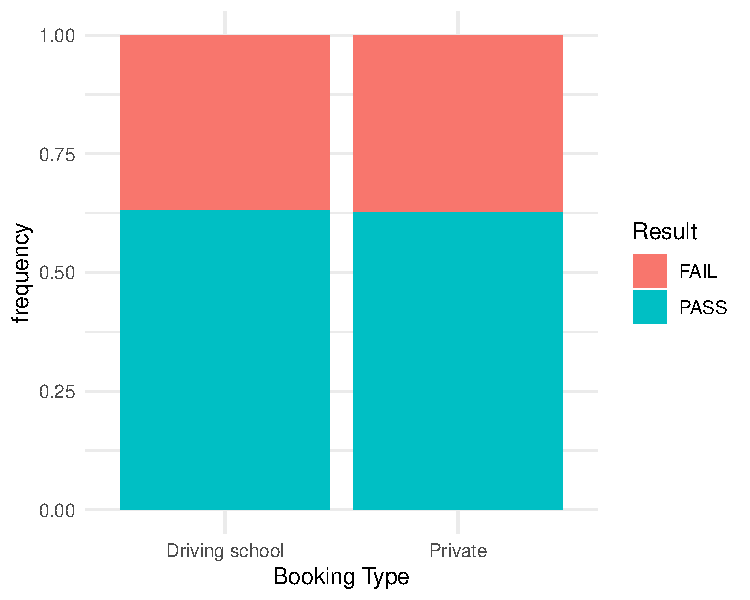
\includegraphics{Assignment4_files/figure-latex/frequency-1} 

}

\caption{Frequency Plot between Booking Type and Exam Result}\label{fig:frequency}
\end{figure}

The frequency plot, Figure \ref{fig:frequency}, between \emph{Booking Type} and \emph{Exam Result} shows that the percentages of people who passed the exam are similar for both driving school and private.

Since the response variable and predictor variable are categorical variables, they will have to be converted into dummy variables(0 \& 1). Then, using logistic regression to analyze their relationship, we get the following equation:

\(Y ~ B(p)\), \(log(\frac{p}{1-p}) = \beta_0 +\beta_1 X + \epsilon\)

\begin{itemize}
\item
  \(\beta_0\) is the intercept.
\item
  \(\beta_1\) is the coefficient of \emph{Booking Type\_Private}
\item
  X is \emph{Booking Type\_Private} taking values 0 or 1
\end{itemize}

\textbackslash begin\{table\}{[}!htbp{]} \centering 
\textbackslash caption\{Regression with \emph{Booking Type\_Private}\}
\label{tab1}

\begin{tabular}{@{\extracolsep{5pt}}lD{.}{.}{-3} } 
\\[-1.8ex]\hline 
\hline \\[-1.8ex] 
 & \multicolumn{1}{c}{\textit{Dependent variable:}} \\ 
\cline{2-2} 
\\[-1.8ex] & \multicolumn{1}{c}{`Exam Result\_PASS`} \\ 
\hline \\[-1.8ex] 
 `Booking Type\_Private` & -0.061^{***} \\ 
  & (0.008) \\ 
  & \\ 
 Constant & 0.559^{***} \\ 
  & (0.006) \\ 
  & \\ 
\hline \\[-1.8ex] 
Observations & \multicolumn{1}{c}{252,813} \\ 
Log Likelihood & \multicolumn{1}{c}{-166,739.600} \\ 
Akaike Inf. Crit. & \multicolumn{1}{c}{333,483.300} \\ 
\hline 
\hline \\[-1.8ex] 
\textit{Note:}  & \multicolumn{1}{r}{$^{*}$p$<$0.1; $^{**}$p$<$0.05; $^{***}$p$<$0.01} \\ 
\end{tabular}

\textbackslash end\{table\}
Table \ref{tab:regression1} shows the regression summary. \emph{Booking Type\_Private} has p-value close to 0 which means it is statistically significant. Due to the variable being a dummy variable relative to booking type driving school, the coefficient indicates that \emph{Booking Type\_Private} affects the passing of an exam negatively compared to \emph{Booking Type\_Driving School}. Private booking reduces the log odds by 0.061.

\begin{table}
\centering
\begin{tabular}{l|r|r|r|r|r}
\hline
  & Df & Deviance & Resid. Df & Resid. Dev & Pr(>Chi)\\
\hline
NULL & NA & NA & 252812 & 333534.7 & NA\\
\hline
`Booking Type\_Private` & 1 & 55.47238 & 252811 & 333479.3 & 0\\
\hline
\end{tabular}
\end{table}

A quick run of ANOVA test on the \emph{logmodel} to analyze the table of deviance shows how well the x variable is doing in comparison to the null model. Here we can see that the drop in deviance is quite small despite having low p-value. We try to improve the model by adding more variables to the function:

\(Y ~ B(p)\), \(log(\frac{p}{1-p}) = \beta_0 +\beta_1 X_1 +\beta_2 X_2 + \epsilon\)

\(X_2\) is \emph{Number of Examinations} taken by each examinee.

The regression with \emph{Number of Examinations} has AIC of 333404. It is slightly lower than the AIC of the previous regression which was 333483. In comparison, having this one extra variable improved the function significantly (statistically).

\begin{table}[!htbp] \centering 
  \caption{Regression Results} 
  \label{} 
\begin{tabular}{@{\extracolsep{5pt}}lD{.}{.}{-3} D{.}{.}{-3} } 
\\[-1.8ex]\hline 
\hline \\[-1.8ex] 
 & \multicolumn{2}{c}{\textit{Dependent variable:}} \\ 
\cline{2-3} 
\\[-1.8ex] & \multicolumn{2}{c}{`Exam Result\_PASS`} \\ 
\\[-1.8ex] & \multicolumn{1}{c}{(1)} & \multicolumn{1}{c}{(2)}\\ 
\hline \\[-1.8ex] 
 `Booking Type\_Private` & -0.061^{***} & -0.060^{***} \\ 
  & (0.008) & (0.008) \\ 
  & & \\ 
 `Number of Examinations` &  & 0.003^{***} \\ 
  &  & (0.0003) \\ 
  & & \\ 
 Constant & 0.559^{***} & 0.542^{***} \\ 
  & (0.006) & (0.006) \\ 
  & & \\ 
\hline \\[-1.8ex] 
Observations & \multicolumn{1}{c}{252,813} & \multicolumn{1}{c}{252,813} \\ 
Log Likelihood & \multicolumn{1}{c}{-166,739.600} & \multicolumn{1}{c}{-166,699.100} \\ 
Akaike Inf. Crit. & \multicolumn{1}{c}{333,483.300} & \multicolumn{1}{c}{333,404.200} \\ 
\hline 
\hline \\[-1.8ex] 
\textit{Note:}  & \multicolumn{2}{r}{$^{*}$p$<$0.1; $^{**}$p$<$0.05; $^{***}$p$<$0.01} \\ 
\end{tabular} 
\end{table}

\begin{tabular}{l}
\hline
x\\
\hline
\\
\hline
\textbackslash{}begin\{table\}[!htbp] \textbackslash{}centering\\
\hline
\textbackslash{}caption\{Regression Results\}\\
\hline
\textbackslash{}label\{\}\\
\hline
\textbackslash{}begin\{tabular\}\{@\{\textbackslash{}extracolsep\{5pt\}\}lD\{.\}\{.\}\{-3\} D\{.\}\{.\}\{-3\} \}\\
\hline
\textbackslash{}\textbackslash{}[-1.8ex]\textbackslash{}hline\\
\hline
\textbackslash{}hline \textbackslash{}\textbackslash{}[-1.8ex]\\
\hline
\& \textbackslash{}multicolumn\{2\}\{c\}\{\textbackslash{}textit\{Dependent variable:\}\} \textbackslash{}\textbackslash{}\\
\hline
\textbackslash{}cline\{2-3\}\\
\hline
\textbackslash{}\textbackslash{}[-1.8ex] \& \textbackslash{}multicolumn\{2\}\{c\}\{`Exam Result\textbackslash{}\_PASS`\} \textbackslash{}\textbackslash{}\\
\hline
\textbackslash{}\textbackslash{}[-1.8ex] \& \textbackslash{}multicolumn\{1\}\{c\}\{(1)\} \& \textbackslash{}multicolumn\{1\}\{c\}\{(2)\}\textbackslash{}\textbackslash{}\\
\hline
\textbackslash{}hline \textbackslash{}\textbackslash{}[-1.8ex]\\
\hline
`Booking Type\textbackslash{}\_Private` \& -0.061\textasciicircum{}\{***\} \& -0.060\textasciicircum{}\{***\} \textbackslash{}\textbackslash{}\\
\hline
\& (0.008) \& (0.008) \textbackslash{}\textbackslash{}\\
\hline
\& \& \textbackslash{}\textbackslash{}\\
\hline
`Number of Examinations` \&  \& 0.003\textasciicircum{}\{***\} \textbackslash{}\textbackslash{}\\
\hline
\&  \& (0.0003) \textbackslash{}\textbackslash{}\\
\hline
\& \& \textbackslash{}\textbackslash{}\\
\hline
Constant \& 0.559\textasciicircum{}\{***\} \& 0.542\textasciicircum{}\{***\} \textbackslash{}\textbackslash{}\\
\hline
\& (0.006) \& (0.006) \textbackslash{}\textbackslash{}\\
\hline
\& \& \textbackslash{}\textbackslash{}\\
\hline
\textbackslash{}hline \textbackslash{}\textbackslash{}[-1.8ex]\\
\hline
Observations \& \textbackslash{}multicolumn\{1\}\{c\}\{252,813\} \& \textbackslash{}multicolumn\{1\}\{c\}\{252,813\} \textbackslash{}\textbackslash{}\\
\hline
Log Likelihood \& \textbackslash{}multicolumn\{1\}\{c\}\{-166,739.600\} \& \textbackslash{}multicolumn\{1\}\{c\}\{-166,699.100\} \textbackslash{}\textbackslash{}\\
\hline
Akaike Inf. Crit. \& \textbackslash{}multicolumn\{1\}\{c\}\{333,483.300\} \& \textbackslash{}multicolumn\{1\}\{c\}\{333,404.200\} \textbackslash{}\textbackslash{}\\
\hline
\textbackslash{}hline\\
\hline
\textbackslash{}hline \textbackslash{}\textbackslash{}[-1.8ex]\\
\hline
\textbackslash{}textit\{Note:\}  \& \textbackslash{}multicolumn\{2\}\{r\}\{\$\textasciicircum{}\{*\}\$p\$<\$0.1; \$\textasciicircum{}\{**\}\$p\$<\$0.05; \$\textasciicircum{}\{***\}\$p\$<\$0.01\} \textbackslash{}\textbackslash{}\\
\hline
\textbackslash{}end\{tabular\}\\
\hline
\textbackslash{}end\{table\}\\
\hline
\end{tabular}

// end of logistic regression model testing

\begin{verbatim}
## 
##  Pearson's Chi-squared test with Yates' continuity correction
## 
## data:  drive$`Booking Type` and drive$`Exam Result`
## X-squared = 6.2967, df = 1, p-value = 0.0121
\end{verbatim}

However, when we run a chi-square test, the p-value is 0.0121 so we have statistical evidence that there is a relationship between \emph{Booking Type} and \emph{Exam Result}.

\begin{center}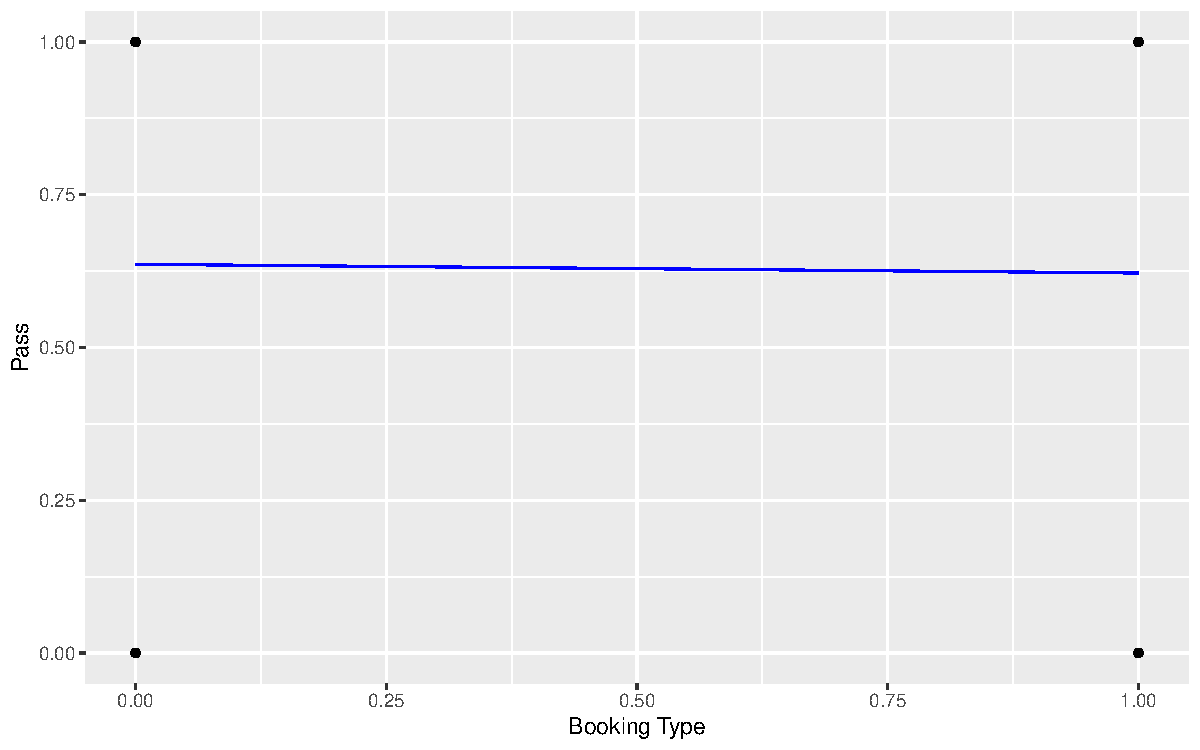
\includegraphics{Assignment4_files/figure-latex/plot_bookingtype_model-1} \end{center}

\printbibliography

\end{document}
